% Matt Mollison
% matt.mollison@gmail.com

\documentclass[12pt]{article}
\usepackage[letterpaper, landscape, margin=1.1in]{geometry} % showframe
\usepackage{wallpaper}
\usepackage{enumitem}

\usepackage{graphicx}

\usepackage{multirow}

% move the level-2 items to the left
\setlist[itemize,2]{leftmargin=10pt}

% don't hyphenate
% \hyphenpenalty=10000
% \raggedright

\begin{document}

\pagestyle{empty}
\centering

% # add border and make background white for potrace
% convert hops_upper_left.png -background white -gravity center -extent 587x382 hops_upper_left_border.png
% convert hops_lower_right.png -background white -gravity center -extent 587x382 hops_lower_right_border.png

% # convert to pnm
% convert hops_upper_left_border.png hops_upper_left_border.pnm
% convert hops_lower_right_border.png hops_lower_right_border.pnm
% # smooth with potrace
% potrace -b pdf -i -o hops_upper_left_border.pdf hops_upper_left_border.pnm
% potrace -b pdf -i -o hops_lower_right_border.pdf hops_lower_right_border.pnm

\ThisULCornerWallPaper{.4}{./img/hops_upper_left_border.pdf}
\ThisLRCornerWallPaper{.4}{./img/hops_lower_right_border.pdf}

% \textsc{{\LARGE Ceremony Program}
% \vspace*{\fill}

\textsc{\LARGE Alice \& Matt}
% \vspace*{\fill}
\vspace*{.2in}

% \textsc{\large Flagstaff Mountain Sunrise Amphitheater}
% % \vspace*{\fill}
% \vspace*{.01in}

\textsc{\large Boulder, CO}
% % \vspace*{\fill}
\vspace*{.01in}

\textsc{\large June 27, 2015}
% \vspace*{\fill}
\vspace*{.25in}

\begin{minipage}[t]{0.495\textwidth}
\centering

\textsc{Order Of Ceremony}

\begin{itemize}

\item [] \textsc{Processional}
\item [] \textsc{Officiant's Welcome}
\item [] \textsc{Community Greeting}
\item [] \textsc{Reading}: An excerpt from \underline{Corelli's Mandolin} by Louis de Berniere
\begin{itemize}[topsep=-5pt,itemsep=-1ex,partopsep=1ex,parsep=1ex]
\item [] \textit{read by Rich Ware}
\end{itemize}

\item [] \textsc{Home Brewing Unity Ceremony}
\begin{itemize}[topsep=-5pt,itemsep=-1ex,partopsep=1ex,parsep=1ex]
\item [] \textit{performed by Wade Mollison and Paul Ware}
\end{itemize}

\item [] \textsc{Reading}: Goodridge \textit{v.} Department of Public Health
\begin{itemize}[topsep=-5pt,itemsep=-1ex,partopsep=1ex,parsep=1ex]
\item [] \textit{read by Kate Mollison}

\end{itemize}

% Marriage is a vital social institution. The exclusive commitment of two individuals to each other nurtures love and mutual support; it brings stability to our society. For those who choose to marry, and for their children, marriage provides an abundance of legal, financial, and social benefits. In return it imposes weighty legal, financial, and social obligations.
%
% Without question, civil marriage enhances the ``welfare of the community.'' It is a ``social institution of the highest importance.''
%
% Civil marriage is at once a deeply personal commitment to another human being and a highly public celebration of the ideals of mutuality, companionship, intimacy, fidelity, and family. Because it fulfills yearnings for security, safe haven, and connection that express our common humanity, civil marriage is an esteemed institution, and the decision whether and whom to marry is among life's momentous acts of self-definition.

\item [] \textsc{Vows \& Ring Ceremony}
\item [] \textsc{Pronouncement}
\item [] \textsc{Recessional}
\end{itemize}

\end{minipage}
\begin{minipage}[t]{0.495\textwidth}
\centering

\vspace*{.23in}
% \textsc{Wedding Party}

\begin{itemize}

\item [] \textsc{Parents of the Bride And Groom}
\begin{itemize}[topsep=-5pt,itemsep=-1ex,partopsep=1ex,parsep=1ex]
\item [] Rich \& Marian Ware
\item [] Mark \& Kelly Mollison
\end{itemize}

\item [] \textsc{Bridal Brigade}
\begin{itemize}[topsep=-5pt,itemsep=-1ex,partopsep=1ex,parsep=1ex]
\item [] Molly Stuhlsatz, Kate Mollison, Sarah Zebrowski, 
Dana Van Oostenburg, Molly Feider
\end{itemize}

\item [] \textsc{Groom's Crew}
\begin{itemize}[topsep=-5pt,itemsep=-1ex,partopsep=1ex,parsep=1ex]
\item [] Fabi\a'an Ca\~{n}as, Wade Mollison, Anthony Helmstetter, 
Adam Bramoweth, Lauren Widelitz
\end{itemize}

\item [] \textsc{Flower Girls}
\begin{itemize}[topsep=-5pt,itemsep=-1ex,partopsep=1ex,parsep=1ex]
\item [] Adeline \& Eleanor Stuhlsatz
\end{itemize}

\item [] \textsc{Instrumentalist}
\begin{itemize}[topsep=-5pt,itemsep=-1ex,partopsep=1ex,parsep=1ex]
\item [] Fabi\a'an Ca\~{n}as, playing a Mountain Goats medley of his own arrangement
\end{itemize}

\item [] \textsc{Officiant}
\begin{itemize}[topsep=-5pt,itemsep=-1ex,partopsep=1ex,parsep=1ex]
\item [] Paloma Ca\~{n}as
\end{itemize}

\end{itemize}
\end{minipage}

\vspace*{\fill}

\newpage

\begin{tabular}{cccc}
\multicolumn{4}{c}{Data mined from our text messages} \\
\includegraphics[width=.55\textwidth]{./img/texts_count.png} & \multicolumn{3}{c}{\raisebox{2.8in}{Most used emojis!}} \\
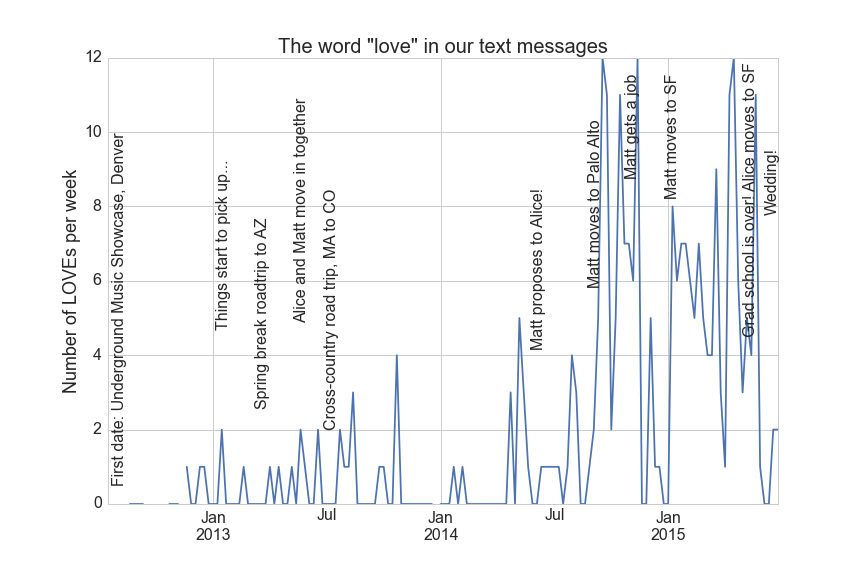
\includegraphics[width=.55\textwidth]{./img/texts_love.png} &
\multirow{2}{*}[5.8in]{\includegraphics[width=.1\textwidth]{./img/emoji_both.png}} &
\multirow{2}{*}[5.8in]{\includegraphics[width=.0667\textwidth]{./img/emoji_alice.png}} &
\multirow{2}{*}[5.8in]{\includegraphics[width=.065\textwidth]{./img/emoji_matt.png}} \\
\end{tabular}

% \begin{tabular}{ccccc}
% & & \multicolumn{3}{c}{Emoji usage! :)} \\
% \includegraphics[width=.5\textwidth]{/Users/matt/src/iphone-sms-backup/data/texts_count.png} & \includegraphics[width=.4\textwidth]{/Users/matt/src/iphone-sms-backup/data/wordcloud_alice.png} \\
% \includegraphics[width=.5\textwidth]{/Users/matt/src/iphone-sms-backup/data/texts_love_normalized.png} &
% \includegraphics[width=.4\textwidth]{/Users/matt/src/iphone-sms-backup/data/wordcloud_matt.png} &
% \multirow{2}{*}[5.35in]{\includegraphics[width=.1\textwidth]{/Users/matt/src/iphone-sms-backup/data/emoji_both.png}} &
% \multirow{2}{*}[5.35in]{\includegraphics[width=.0667\textwidth]{/Users/matt/src/iphone-sms-backup/data/emoji_alice.png}} &
% \multirow{2}{*}[5.35in]{\includegraphics[width=.065\textwidth]{/Users/matt/src/iphone-sms-backup/data/emoji_matt.png}} \\
% \end{tabular}

\end{document}
